\documentclass[twoside]{article}
\usepackage{amsmath,amsthm,amssymb,amsfonts,amscd}
\usepackage{url}
\usepackage[spanish,english]{babel}
%%%%%%%%%%%%%%%%%%%%%%%%%%%%%%%%%%%
% Compilar figuras
%%%%%%%%%%%%%%%%%%%%%%%%%%%%%%%%%
\usepackage{graphics}
\usepackage{epsfig}
\usepackage{graphicx}
\usepackage{float} %Coloca las imagenes justo en el lugar donde se desea con el
                   %comando \begin{figure}[H]
\usepackage{subfigure} %permite agregar subfiguras
\usepackage{epstopdf}
%%%%%%%%%%%%%%%%%%%%%%%%%%%%%%%%%%%
% Acentuación y símbolos en español
%%%%%%%%%%%%%%%%%%%%%%%%%%%%%%%%%%%
\usepackage[utf8x]{inputenc}
%%%%%%%%%%%%%%%%%%%%%%%%%%%%%%%%%%%
\usepackage{fancyhdr}
\textwidth 35pc
\textheight 47pc
\oddsidemargin 1.5pc
\evensidemargin 1.5pc
\voffset -1pc
\renewcommand{\thefootnote}{}
\setcounter{page}{1} %*** # primera pagina***
\fancypagestyle{plain}{\fancyhf{}%
\fancyhead[L]{\footnotesize{Nombre de la Revista Vol. XX, No. X (20XX), pp. \pageref{begin-art}--\pageref{end-art} \vspace{-6mm} \begin{flushright}
 p-ISSN XXXX-XXXX                                                                                                                                                                                                                             \end{flushright}
}}%
\renewcommand{\headrulewidth}{0pt}\renewcommand{\footrulewidth}{0pt}}

\fancypagestyle{headings}{\fancyhf{}%
\renewcommand{\headrulewidth}{0.4pt}%
\renewcommand{\footrulewidth}{0.4pt}%
\fancyhead[LE,RO]{\thepage}%
\fancyhead[RE]{Rodrigo Antonio Gómez Hernández}%
\fancyhead[LO]{PredStock (Stock Market Prediction)}%
\fancyfoot[C]{\footnotesize{Nombre de la Revista Vol. XX, No. X (20XX), pp. \pageref{begin-art}--\pageref{end-art}}}}


%%%%%%%%%%%%%%%%%%%%%%%%%%%%%%%%%%
% Declaraciones, nuevos comandos, etc.%
%%%%%%%%%%%%%%%%%%%%%%%%%%%%%%%%%%
\newtheorem{teo}{Teorema}[section]
\newtheorem{propo}{Proposici\'on}[section]
\newtheorem{lema}{Lema}[section]
\newtheorem{corl}{Corolario}[section]
\theoremstyle{definition}
\newtheorem{defi}{Definici\'on}[section]
\theoremstyle{example}
\newtheorem{ejem}{Ejemplo}[section]
\theoremstyle{remark}
\newtheorem{nota}{Nota}[section]
%%%%%%%%%%%%%%%%%%%%%%%%%%%%%%%%%%%%%%%
% Enumeración de ecuaciones
%%%%%%%%%%%%%%%%%%%%%%%%%%%%%%%%%%%%%%%
\renewcommand{\theequation}{\thesection.\arabic{equation}}
\numberwithin{equation}{section}%%%%%%%%%%%%%%%%%%%%%%%%%%%%%


\begin{document}
\label{begin-art}
\pagestyle{headings}
\thispagestyle{plain} 
\footnote{\hspace{-18.1pt} Recibido ***. Revisado ***.
Aceptado ***. Publicado en línea: *** \\ MSC (2010): Primary ****; Secondary ****.\\ Autor de correspondencia: Nombre del autor de correspondencia}
\selectlanguage{spanish}
\begin{center}
{\LARGE\bfseries PredStock (Stock Market Prediction) \\
Comparación entre modelos paramétricos y no paramétricos para la predicción de 21 índices bursátiles\par }

\vspace{5mm}
{\large Rodrigo Antonio Gómez Hernández (\url{rdgomezh@unbosque.edu.co})}\\
Departamento de Matemáticas y Estadística, Facultad de Ciencias\\
Universidad El Bosque\\
Bogotá D.C., Colombia

\vspace{3mm}
{\large Director: Héctor Javier Hortúa Orjuela (\url{hhortuao@unbosque.edu.co})}\\
Departamento de Matemáticas y Estadística, Facultad de Ciencias\\
Universidad El Bosque\\
Bogotá D.C., Colombia

\end{center}
\vspace{5mm}

\begin{abstract}
 En este artículo se comparan los resultados de los modelos utilizados en la predicción de diferentes índices bursátiles y que hacen parte de los modelos de predicción utlizados en un WebSite cuyo nombre de dominio es idéntico al de este artículo. Se encontrará una breve descripción de dichos modelos entre ellos los modelos paramétricos de series de tiempo (ARMA, ARIMA, SARIMA, entre otros) y modelos no paramétricos como los modelos de redes neuronales de corta memoria LSTM, modelos de capas densas y redes neuronales bayesianas, entre otros. \\
 
{\bf Palabras y frases clave:} Predicción, modelos paramétricos, modelos no paramétricos.
\end{abstract}

\selectlanguage{english}

\begin{abstract}
 This article compares the results of the models used in the prediction of different stock actions and that are part of the prediction models used in a website whose domain name is identical to the one in this article. See a brief description of these models, including parametric time series models (ARMA, ARIMA, SARIMA, among others) and non-parametric models such as LSTM short memory neural network models, dense layer models, and Bayesian neural networks, among others.\\
 
{\bf Key words and phrases:} Forecast, paramétric models, non-parametric models.
\end{abstract}

\selectlanguage{spanish}

\section{Introducci\'on}
  Una de las principales tareas de la estadística es la es no quedarse solamente en la descripción de los datos que a lo largo del tiempo se han recogido, sino además buscar entre estos datos tendencias y repeticiones cíclicas que permitan contestar la interrogante “¿qué sucederá después?”\cite{7}. Con esto en mente la evolución de los modelos a modelos más complejos y las evolución herramientas de cómputo ha permitido crear modelos matemáticos capaces de arrojar una mayor precisión pero con un costo computacional más elevado.  Específicamente en relación a los valores que arrojan los índices bursátiles, se caracterizan por ser valores aleatorios que dependen de múltiples factores (económicos, macroeconómicos, políticos, geográficos, atmosféricos, etc.), factores que son imposible de controlar a la vez, además son valores que pueden cambiar rápidamente en el transcurso de un día, obedeciendo a la ley de oferta y demanda\cite{4}. El atractivo de este mercado en la actualidad es la facilidad con la que un usuario cualquiera con una capacidad de inversión no muy grande, puede realizar transacciones en uno de los muchos WebSite dedicados a este fin y obtener un margen de ganancia favorable (por lo general mayor a los que un CDT o Bono bancario puede generar), con un riesgo proporcional al porcentaje de ganancia. 
  
En este artículo se muestra los resultados (junto a una breve descripción de los  modelos utilizados),generados por modelos paramétricos de series de tiempo (ARMA, ARIMA, SARIMA, SARIMAX, ARIMAX y ARMAX), modelos de carácter no paramétrico como los generados por Redes Neuronales de corta memoria (LSTM), modelos de capas densa y convolucionales y modelos de redes neuronales bayesianas. 

Los modelos ya descritos se utilizarán para predecir 21 de los principales índices bursátiles de todo el mundo; 8 de Europa, 7 de Asía y 6 de América cuyos datos se registran diariamente (exceptuando los días festivos) desde 2019 hasta el presente. Cabe destacar que los datos son tomados de una fuente confiable\cite{5}. Una vez tratados los datos se procede a calibrar los modelos para cada índice y determinar sobre el índice la precisión del modelo en su papel predictivo. 

Surgen entonces la interrogante ¿Habrá un modelo en particular capaz de dar la mejor predicción a los 21 índices bursátiles o por el contrario serán diferentes modelos los que arrojen las mejores predicciones en los diferentes índices?

 
\section{Objetivos}
\subsection{Objetivo General}
Crear un WebSite que permita a los usuarios visualizar las tendencias y predicciones de los principales índices bursátiles (stock-exchange), a través de modelos estadísticos paramétricos, algoritmos no paramétricos como LSMT y NNB\cite{1,2}, dependiendo de su capacidad predictiva.

Realizar una comparación de las predicciones de modelos para forecasting paramétricos y no paramétricos como LSMT y NNB para la predicción de 21 índices bursátiles, a través de sus métricas de ajuste y pérdida.
 
\subsection{Objetivos Específicos}
Crear y automatizar los diferentes modelos de predicción con alta capacidad de predicción y baja funciones de pérdida, para los stock seleccionados por el usuario, con ayuda de las métricas de ajuste y comportamiento a través del tiempo.

Construir un back-end robusto que permita la mayor eficiencia de recursos tanto en la recolección de la información como en la generación de estimaciones.

Construir un Front-end atractivo y amigable para el usuario, cuya interacción sea intuitiva y que personas con pocos conocimientos econométricos y financieros sean capaces de disernir tendencias que les permitirán tomar decisiones de compra o venta de las acciones.

\section{Metodología}
  Referente al artículo se tomarán cada uno de los 21 índices bursátiles y se ajustarán cada uno de los modelos propuestos para cada uno de los índices, se tomarán las métricas de ajuste y pérdida como criterio de comparación. Junto con esto se evaluará cuantificará la incertidumbre de cada modelo a través del porcentaje de datos reales (de un subconjunto de prueba) de que están en los límites arrojados de cada modelo. 

\begin{figure}[ht]
  \centering
  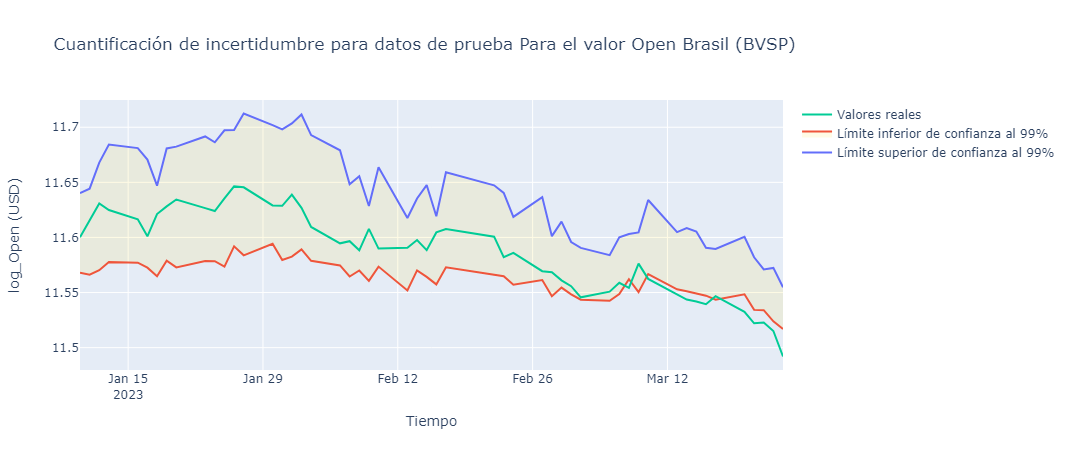
\includegraphics[width=1.0\textwidth]{Brasil.png}
  \caption{Índice bursátil IBOVESPA (Brasil) predicción de intervalo con BNN}
\end{figure}

\section{Referencias}

\begin{thebibliography}{99}
%%%% Artículos %%%%%%%%%%%%%%%%%%%%%%%%%%%%%%%%%%%%%%%%%%%%%%%%%%%%%%%%
\bibitem{1} L. Perreault Levasseur, Y. D. Hezaveh, and R. H. Wechsler,Uncertainties in Parameters Estimated with Neural Networks: Application to Strong Gravitational Lensing, Astrophys. J. 850, L7 (2017), arXiv:1708.08843 [astroph.CO].

\bibitem{2} H.J. Hortúa, R. Volpi, D. Marinelli and L. Malagó,
Parameters Estimation for the Cosmic Microwave Background with Bayesian Neural Networks, arXiv:1911.08508v3 [astro-ph.IM] 30 Oct 2020.

\bibitem{3} A. Gautam and V. Singh, Parametric Versus Non-Parametric Time Series Forecasting Methods: A Review, Journal of Engineering Science and Technology Review 13 (3) (2020) 165 - 171, 22 May 2020.

\bibitem{4} M. C. García, A. M. Jalal, L. A. Garzón y J. M. López, Métodos para predecir índices bursátiles, Ecos de Economía ISSN 1657-4206 I Año 17 I No. 37 I julio-diciembre 2013 I pp. 51-82 I Medellín-Colombia.


%%% Página web %%%%%%%%%%%%%%%%%%%%%%%%%%%%%%%%%%%%%%%%%%%%%%%%%%%%%%%%
\bibitem{5} Yahoo Finance, Histórical Stocks, 2023, 2023-04-12, \url{https://finance.yahoo.com/}.


\bibitem{6} A Gentle Introduction to Time Series Analysis and Forecasting, 2023
\url{https://wandb.ai/iamleonie/A-Gentle-Introduction-to-Time-Series-Analysis-Forecasting/reports/A-Gentle-Introduction-to-Time-Series-Analysis-Forecasting--VmlldzoyNjkxOTMz}.

\bibitem{7} What is predictive analytics?, Google Cloud, 2023
\url{https://cloud.google.com/learn/what-is-predictive-analytics}.

\end{thebibliography}

\label{end-art}
\end{document}
